\begin{frame}
    \begin{block}{Probléme Modéle SIR}
        \begin{itemize}
            \item Chance pour un infecté de propagé l'épidémie est uniforme
            \item Chance de contact avec tous les autres individus est uniforme
        \end{itemize}
    \end{block}

    \begin{center}
        \bf Il nous faut un modéle plus proche de la réalité
    \end{center}
\end{frame}


\begin{frame}
    \frametitle{Reed et Forst}

    \begin{block}{Définition}
        L'infections ménent d'abord à une période infectieuse, puis une période de rétablissement pour aprés finalement finir dans le groupe des immunisés. Les nouvelles infections se produisent par génération, séparées par la période de latence.
    \end{block}

    \begin{itemize}
        \item Le modèle est généralement utilisé avec une dynamique à temps discret, où la période infectieuse est courte et précédée d’une période de latence plus longue.
        \item Les probabilités dans chaque génération dépendent de l’état de l’épidémie dans la génération précédente, et sont spécifiées par des probabilités binomiales.
    \end{itemize}
\end{frame}

\begin{frame}
        \frametitle{Modéle SIR}

        \centering
        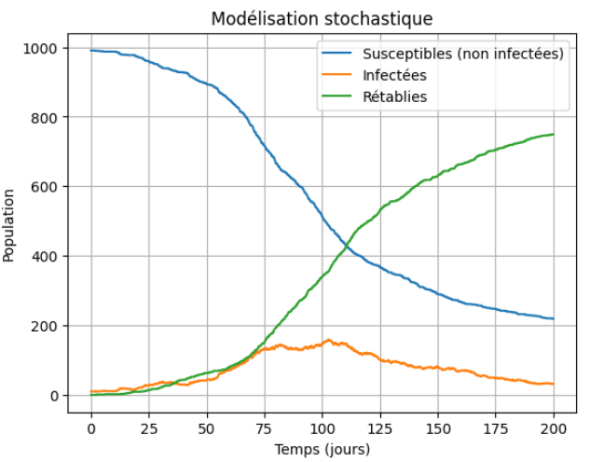
\includegraphics[scale=0.25]{sir_stochastique}

        \begin{itemize}
                \item $\gamma = 0.05$
                \item $\beta = 0.1$
                \item $N = 1000$
                \item $I_0 = 10$
        \end{itemize}

\end{frame}

\begin{frame}
    \frametitle{Reed et Forst}

    \begin{alertblock}{Loi Binomiale}
        $$ P(X = k) = \binom{n}{k}p^k(1 - p)^{n-k} $$
    \end{alertblock}

    \begin{itemize}
        \item La loi Binomiale est la loi suivis par la variable aléatoire X qui compte le nombre de succés de n expériences de Bernouli consécutives et indépendantes.
        \item La loi de Bernouli est la loi suivis par l'expérience qui peut résussir avec une probabilités p.
    \end{itemize}
\end{frame}

\begin{frame}
    \frametitle{Reed et Forst}

    \begin{alertblock}{Définition}
        \begin{align}
            P &= P(Y_{j+1} = y_{j+1} | X_0 = x_0, Y_0 = y_0, ..., X_j = x_j, Y_j = y_j) \\
              &= P(Y_{j+1} = y_{j+1} | X_j = x_j, Y_j = y_j) \\
              &= \binom{x_j}{y_{j+1}}(1 - q^{y_j})^{y_{j+1}}(q^{y_j})^{x_j - y_{j+1}}
        \end{align}
    \end{alertblock}
\end{frame}
